\section{Specification}
For the specification of \name, we will describe three different kinds of specification. The functionality, interaction and presentation specifications. The functionality specification describes which functions should be possible in \name. The interaction specification describes how the user can interact with the system. The presentation specification describes how \name should look like. 
 \subsection{Functionality}
 The functionality is divided in some different functions and the specification of this functions. Also we have some functionality that should work, with all functions.
 The following functionality should be in the \name, to make it useful.
  \begin{itemize}
  \item There should be at least 2 different kind of building blocks. 
  \item There should some basic physics in which the building blocks behave, so that it is not possible to make very unrealistic scenes.
  \end{itemize}
  There should be default levels, for the user to solve. In this default levels, the users has a standard amount of building blocks, to make the bridge strong enough for a train to ride over it. 
 \begin{itemize}
 \item The user can only use the building blocks defined for the level
 \item It should be possible to make a bridge strong enough for a train to ride over it
 \end{itemize}
  It should be possible for the user to create their own levels, so that other users can try to solve this level. 
 \begin{itemize}
 \item The user has to solve the level himself, before other users can try to solve the level.
 \item Other users can only use the building blocks, that the user used to make a bridge.
 \item The user should be able to change the properties of building blocks, for example they should be able to change the height, width, color and strength.
 \end{itemize}

\subsection{Interaction}
The interaction will be a simple drag and drop system, where the user can select a building block. Then he can drag it too the scene and rotate it in every way. The building blocks will connect through spheres at default places of the building block. As you can see in figure \ref{fig:sbb}, the spheres of the beam building block are on each corner and on the building block of the metal cable, the spheres are at each end of the cable. The two building blocks will connect when the two spheres are dragged closed enough and the user, release the mouse button. So that it does not connect to every sphere that is dragged over, but only to the one that the user wants to connect. 
\begin{figure}[H]
    \centering
    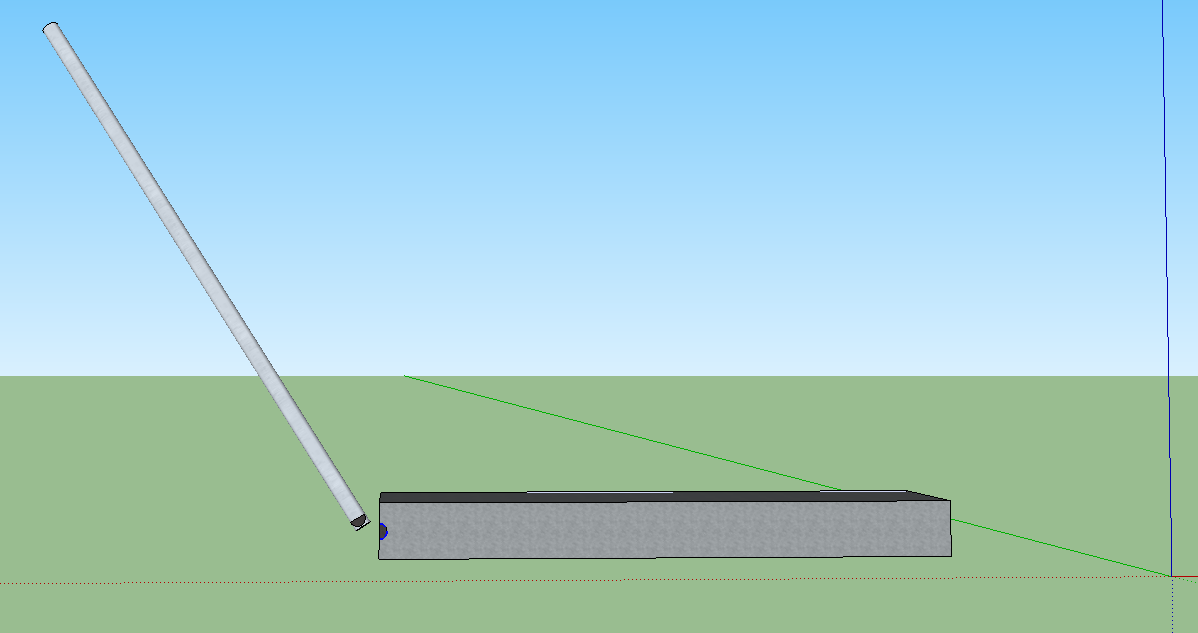
\includegraphics[width=0.8\textwidth]{pics/Spheresbuildingblocks.png}
    \caption{Sample building blocks}
    \label{fig:sbb}
\end{figure}

\subsection{Presentation}
The presentation will be a basic 3D world. The basic 3D world will be a simple ravine, that looks likes figure \ref{fig:rav}. There will be a tool bar on the right to select building blocks.
\begin{figure}[H]
    \centering
    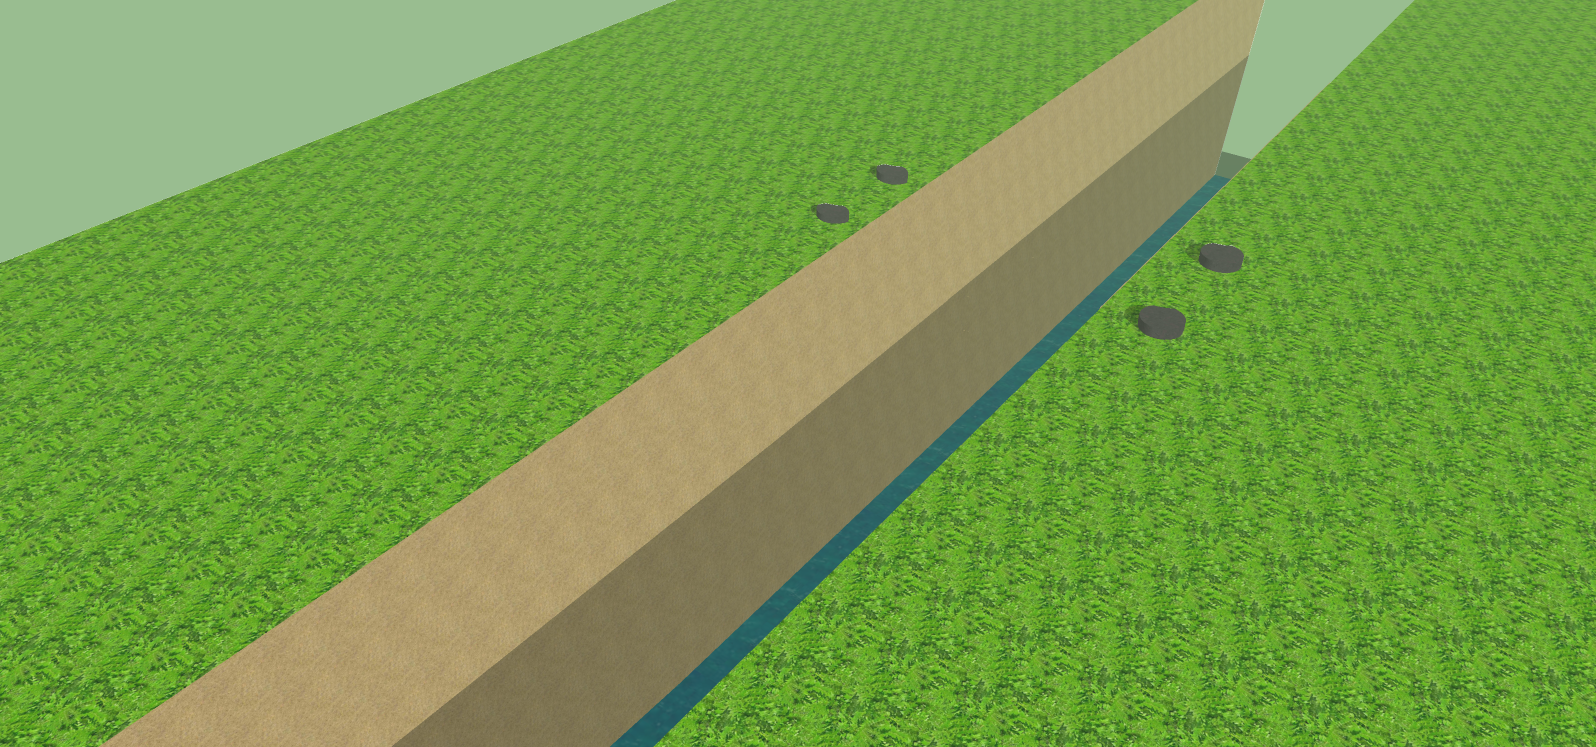
\includegraphics[width=0.8\textwidth]{pics/Ravine.png}
    \caption{Ravine}
    \label{fig:rav}
\end{figure}
 Additional requirements for the presentation:
 \begin{itemize}
 \item Better looking building blocks
 \item More than one 3D world to build bridges in. This could be a over a canal or a river. This could be in different places, like in a city or a mountain.
 \item Customizable 3D world, so that users can change the depth, the width etc. of the ravine. So that users can add rocks to build on in the middle of the ravine.
 \end{itemize}